\chapter{Analysis of processing results}
\label{analysis_processing}

The results of the clustering and matching algorithm where visually reviewed to verify the performance. Thought iterative adjustments of the input parameters the clustering and matching algorithm where calibrated to a sufficient representation level (see final input parameters in \autoref{methodology_detection} and \autoref{methodology_matching}).

\todo{Add Figures of clustering as proof} 

\section{Correlation Processing}

The resulting datasets created by the evaluation tool (see section \autoref{methodology_detection} \ref{methodology_matching} and \ref{methodology_data_processing}), task to detection and cluster jams and find adjacent incidents, are then processed by the correlation tool. The correlation tool creates a matrix table with the correlation coefficients.  This table is visual presented in figure \ref{img:correlation_matrix_matched_cramers} showing the the correlation of each parameters for matched dataset.

% -----------------------------------
% -------- BAYSIS - Matched ---------
% -----------------------------------
\subsection{BAYSIS - Matched}

List of strong correlations (.14 for $\eta$ and 0.5 for $r$ ...):

\newgeometry{left=1.5cm,right=1cm}
	\pagestyle{empty}
	\begin{figure}[ht]
		\centering
		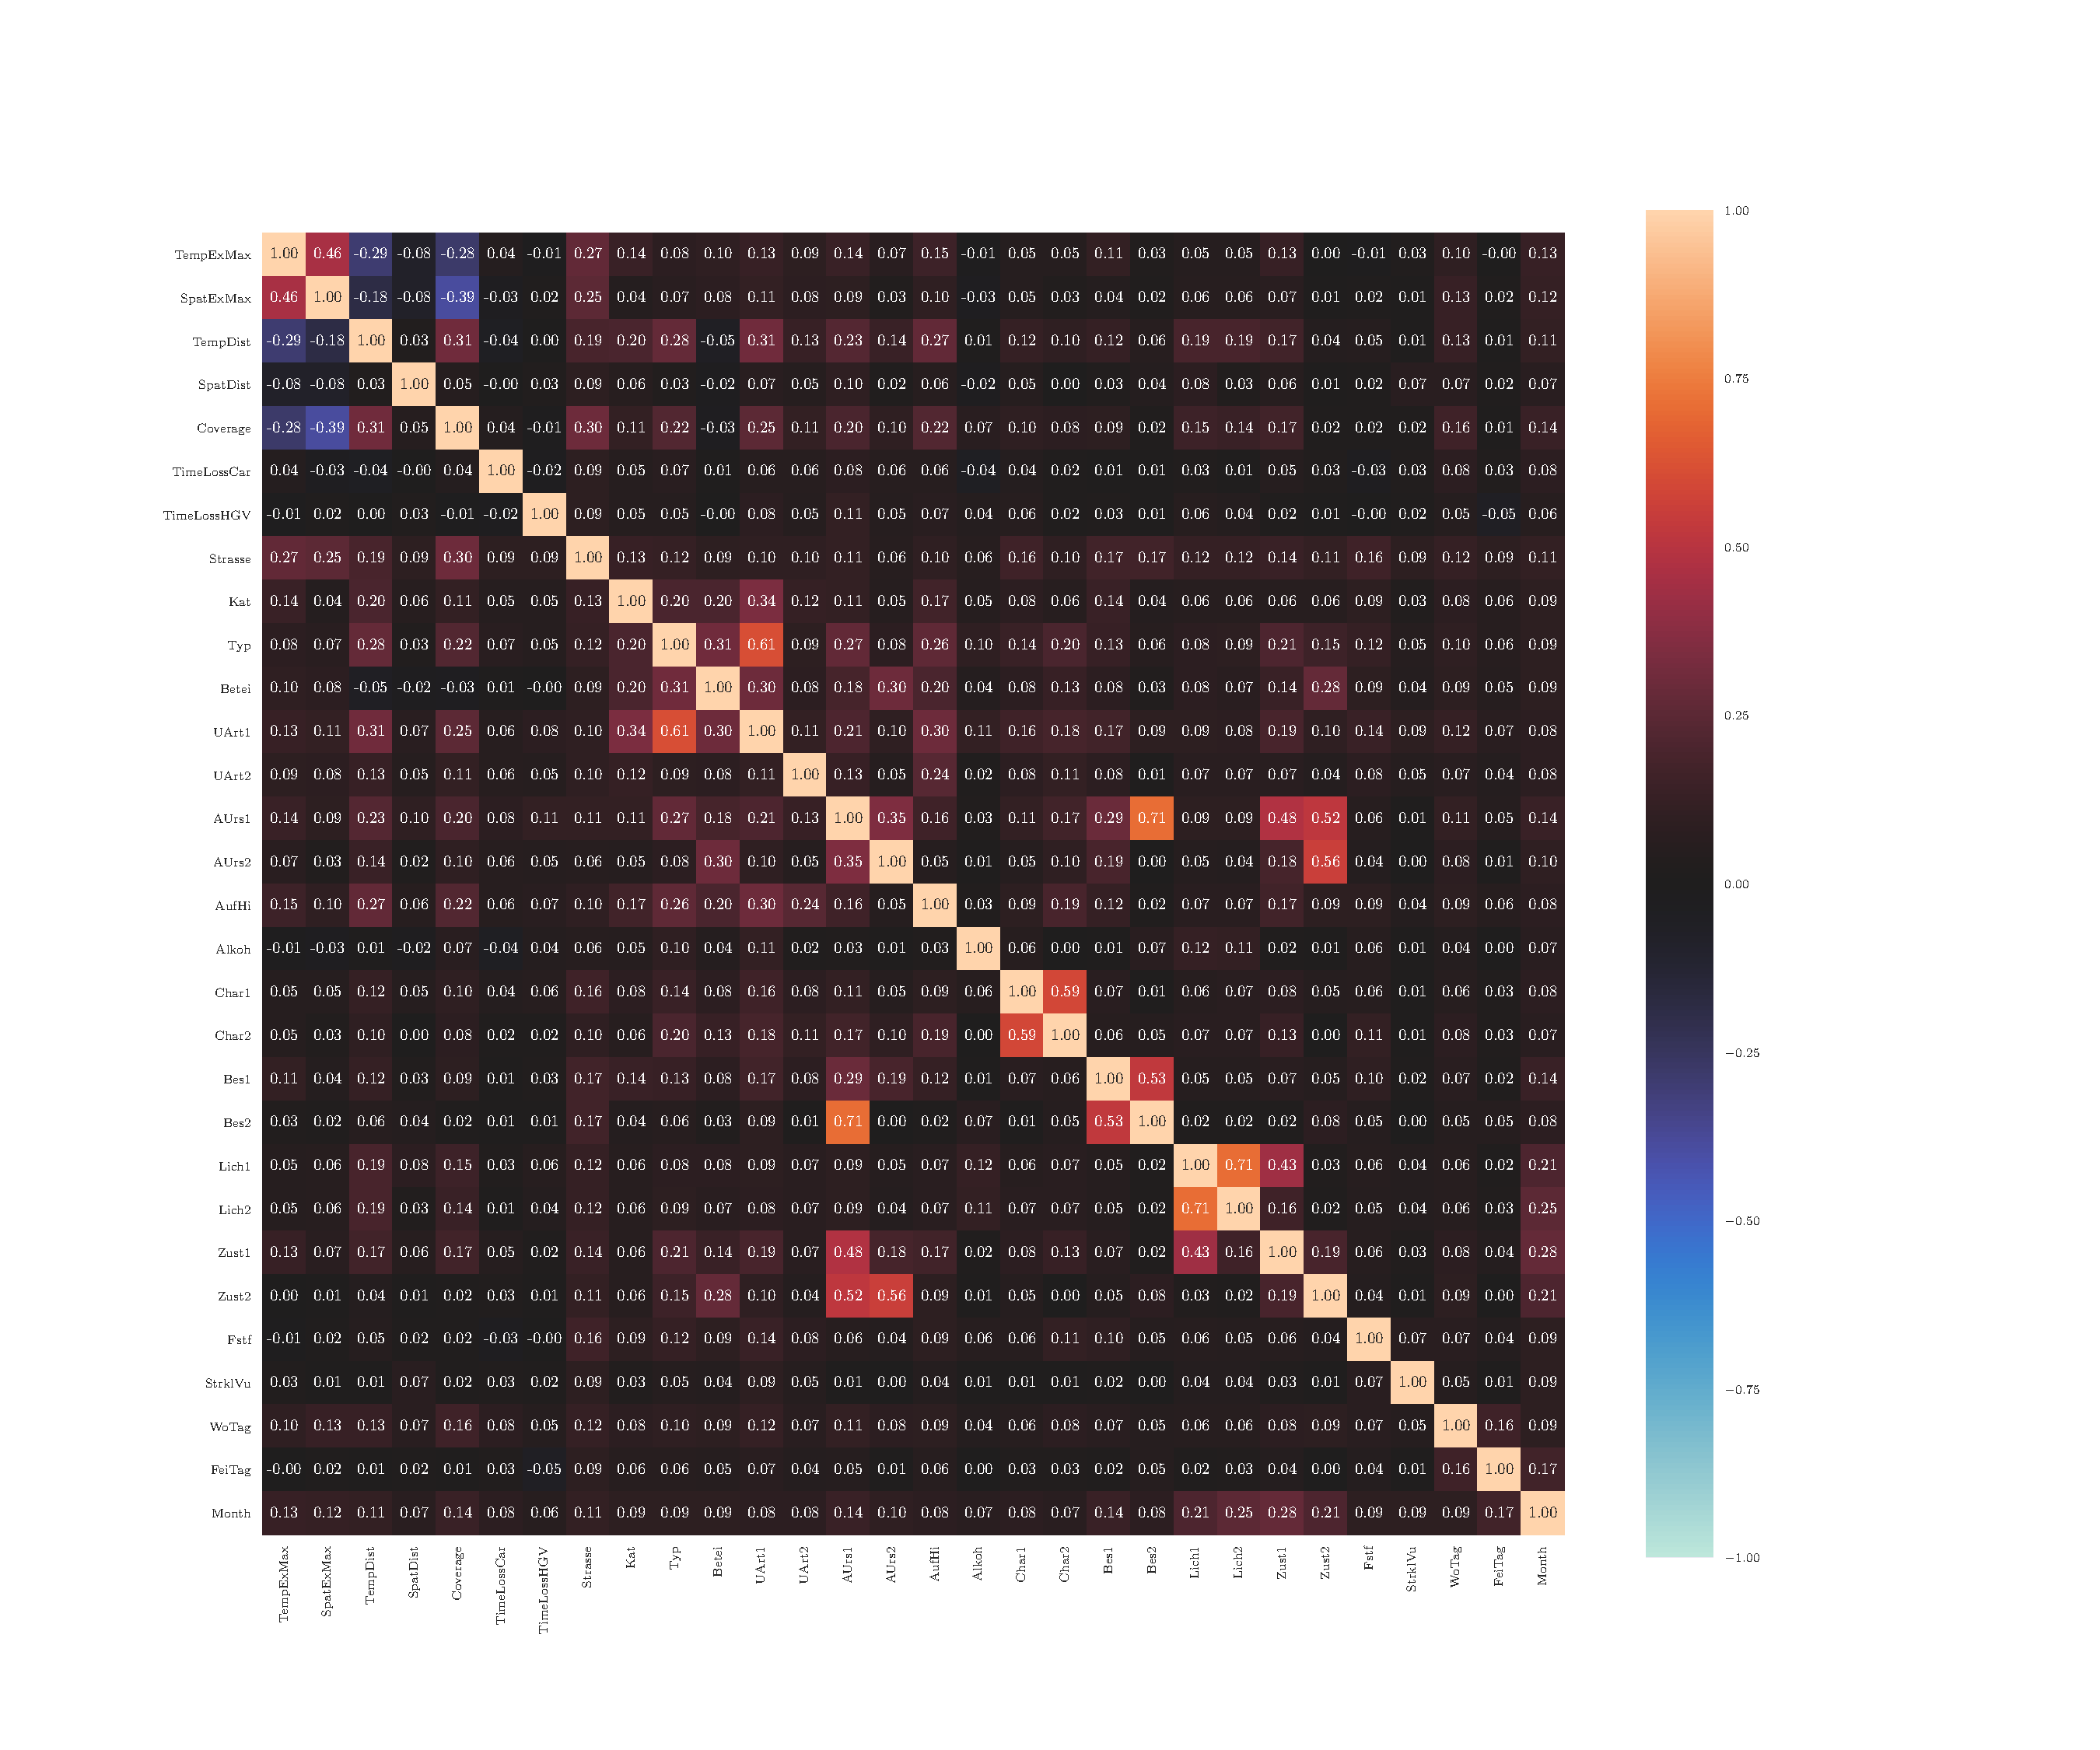
\includegraphics[scale=0.52, trim=3cm 2cm 0cm 0cm]{../CorrAnalysis/data/BAYSIS/02_matched/plots/baysis_matched_corr_cramers}
		\caption{Correlation matrix for BAYSIS matched data, with $V$, $\eta$, $\tau$, $r_{pq}$, $r$}
		\label{img:correlation_matrix_matched_cramers}
	\end{figure}
\restoregeometry
\pagestyle{headings}

\noindent
\begin{table}[ht]
	\centering
	\begin{tabular}{c|l|l}  
		Category & Strong & Moderate \\
		\\[-1em]
		\hline
		\\[-1em]
		Strasse & TMax, TAvg, SMax, SAvg, TDist, SDist, Cov & \\ 
 		Kat & TMax, TAvg, SAvg, TDist & \\ 
 		Typ & TDist, Cov & \\
 		%Betei & & \\
 		UArt1 & SAvg, TDist, Cov & \\
 		%UArt2 & & \\
 		AUrs1 & SAvg, TDist, SDist, Cov, TLHGV & \\
 		%AUrs2 & & \\
 		AufHi & TMax, TAvg, TDist, Cov & \\
 		%Alkoh & & \\
 		%Char1 & & \\
 		%Char2 & & \\
 		%Bes1 & & \\
 		Lich1 & Cov & \\
 		Lich2 & Cov & \\
 		Zust1 & Cov & \\
 		%Zust2 & & \\
 		%Fstf & & \\
 		WoTag & Cov & \\
 		%FeiTag & & \\
 		Month & Cov & \\
	\end{tabular}
	\caption{List of incident variables and their strong/moderated correlated jam variable from the BAYSIS matched data}
\end{table}

Are these correlations significant or not ? --> Wilcoxon Test
\smallskip
Where are the significant correlations? --> Pairwise Test

% --------------------------
% -------- Strasse ---------
% --------------------------
\large
\centerline{\textbf{Strasse}}
\normalsize

\paragraph{Maximal temporal Extent:}

Kruskal-Wallis chi-squared = 324.16, df = 210, p-value = 6.956e-07

\begin{table}[ht]
	\tiny
	\setlength{\tabcolsep}{4pt}
	\centering
	\begin{tabular}{rrrrrrrrrrrrrrrrr}
		\toprule
		& A3 & A6 & A9 & A70 & A96 & A7 & A73 & A99 & A92 & A93 & A94 & A72 & A995 & A95 & A71 & A45 \\ 
		\midrule
		A6 & 0.00 &  &  &  &  &  &  &  &  &  &  &  &  &  &  &  \\ 
		A9 & 0.00 & 1.00 &  &  &  &  &  &  &  &  &  &  &  &  &  &  \\ 
		A70 & 0.01 & 1.00 & 1.00 &  &  &  &  &  &  &  &  &  &  &  &  &  \\ 
		A96 & 0.00 & 1.00 & 0.22 & 1.00 &  &  &  &  &  &  &  &  &  &  &  &  \\ 
		A7 & 0.00 & 1.00 & 1.00 & 1.00 & 1.00 &  &  &  &  &  &  &  &  &  &  &  \\ 
		A73 & 0.00 & 1.00 & 0.31 & 1.00 & 1.00 & 1.00 &  &  &  &  &  &  &  &  &  &  \\ 
		A99 & 1.00 & 1.00 & 1.00 & 1.00 & 0.44 & 1.00 & 0.59 &  &  &  &  &  &  &  &  &  \\ 
		A92 & 0.00 & 1.00 & 0.16 & 1.00 & 1.00 & 1.00 & 1.00 & 0.22 &  &  &  &  &  &  &  &  \\ 
		A93 & 1.00 & 1.00 & 1.00 & 1.00 & 1.00 & 1.00 & 1.00 & 1.00 & 1.00 &  &  &  &  &  &  &  \\ 
		A94 & 0.01 & 1.00 & 1.00 & 1.00 & 1.00 & 1.00 & 1.00 & 1.00 & 1.00 & 1.00 &  &  &  &  &  &  \\ 
		A72 & 1.00 & 1.00 & 1.00 & 1.00 & 1.00 & 1.00 & 1.00 & 1.00 & 1.00 & 1.00 & 1.00 &  &  &  &  &  \\ 
		A995 & 1.00 & 1.00 & 1.00 & 1.00 & 1.00 & 1.00 & 1.00 & 1.00 & 1.00 & 1.00 & 1.00 & 1.00 &  &  &  &  \\ 
		A95 & 1.00 & 1.00 & 1.00 & 1.00 & 1.00 & 1.00 & 1.00 & 1.00 & 1.00 & 1.00 & 1.00 & 1.00 & 1.00 &  &  &  \\ 
		A71 & 1.00 & 1.00 & 1.00 & 1.00 & 1.00 & 1.00 & 1.00 & 1.00 & 1.00 & 1.00 & 1.00 & 1.00 & 1.00 & 1.00 &  &  \\ 
		A45 & 1.00 & 1.00 & 1.00 & 1.00 & 1.00 & 1.00 & 1.00 & 1.00 & 1.00 & 1.00 & 1.00 & 1.00 & 1.00 & 1.00 & 1.00 &  \\ 
		A980 & 1.00 & 1.00 & 1.00 & 1.00 & 1.00 & 1.00 & 1.00 & 1.00 & 1.00 & 1.00 & 1.00 & 1.00 & 1.00 & 1.00 & 1.00 & 1.00 \\ 
		\bottomrule
	\end{tabular}
	\caption{Wilcoxon Pairwise t-test for \textit{Street} by \textit{TempMax}}
\end{table}

\begin{table}[ht]
	\tiny
	\centering
	\begin{tabular}{c|c|c|c|c|c|c|c}
		\toprule
		Group & $n$ & $\bar{x}$ & $\sigma$ & $\tilde{x}$ & $min$ & $max$ & $\Delta$ \\ 
		\midrule
		A3 & 574 & 235.29 & 218.01 & 162.00 & 9.00 & 1323.00 & 1314.00   \\ 
		A6 & 127 & 153.05 & 150.42 & 108.00 & 12.00 & 864.00 & 852.00   \\ 
		A9 & 466 & 170.85 & 151.33 & 118.50 & 9.00 & 1194.00 & 1185.00   \\ 
		A70 & 31 & 106.55 & 79.42 & 81.00 & 24.00 & 369.00 & 345.00   \\ 
		A96 & 156 & 117.94 & 80.93 & 106.50 & 12.00 & 384.00 & 372.00   \\ 
		A7 & 130 & 153.37 & 194.10 & 102.00 & 9.00 & 1341.00 & 1332.00  \\ 
		A73 & 129 & 125.95 & 135.01 & 93.00 & 12.00 & 1323.00 & 1311.00  \\ 
		A99 & 116 & 169.09 & 136.72 & 138.00 & 15.00 & 681.00 & 666.00  \\ 
		A92 & 66 & 103.86 & 65.69 & 87.00 & 18.00 & 354.00 & 336.00 \\ 
		A93 & 21 & 163.57 & 155.71 & 111.00 & 36.00 & 588.00 & 552.00   \\ 
		A94 & 37 & 101.59 & 54.60 & 99.00 & 15.00 & 249.00 & 234.00 \\ 
		A72 & 1 & 60.00 &  & 60.00 & 60.00 & 60.00 & 0.00 \\ 
		A995 & 2 & 28.50 & 27.58 & 28.50 & 9.00 & 48.00 & 39.00   \\ 
		A95 & 4 & 72.00 & 33.50 & 82.50 & 24.00 & 99.00 & 75.00  \\ 
		A71 & 3 & 90.00 & 78.63 & 69.00 & 24.00 & 177.00 & 153.00   \\ 
		A45 & 3 & 103.00 & 52.85 & 96.00 & 54.00 & 159.00 & 105.00   \\ 
		A980 & 1 & 99.00 &  & 99.00 & 99.00 & 99.00 & 0.00   \\ 
 		\bottomrule
	\end{tabular}
	\caption{Group description of Street by TempMax}
\end{table}

\paragraph{Average temporal Extent:}
Kruskal-Wallis rank sum test chi-squared = 324.97, df = 245, p-value = 0.000466

\begin{table}[ht]
	\tiny
	\setlength{\tabcolsep}{4pt}
	\centering
	\begin{tabular}{rrrrrrrrrrrrrrrrr}
		\toprule
		& A3 & A6 & A9 & A70 & A96 & A7 & A73 & A99 & A92 & A93 & A94 & A72 & A995 & A95 & A71 & A45 \\ 
		\midrule
		A6 & 0.55 &  &  &  &  &  &  &  &  &  &  &  &  &  &  &  \\ 
		A9 & 0.17 & 1.00 &  &  &  &  &  &  &  &  &  &  &  &  &  &  \\ 
		A70 & 0.85 & 1.00 & 1.00 &  &  &  &  &  &  &  &  &  &  &  &  &  \\ 
		A96 & 0.04 & 1.00 & 1.00 & 1.00 &  &  &  &  &  &  &  &  &  &  &  &  \\ 
		A7 & 1.00 & 1.00 & 1.00 & 1.00 & 1.00 &  &  &  &  &  &  &  &  &  &  &  \\ 
		A73 & 0.00 & 1.00 & 0.51 & 1.00 & 1.00 & 1.00 &  &  &  &  &  &  &  &  &  &  \\ 
		A99 & 0.01 & 1.00 & 1.00 & 1.00 & 1.00 & 1.00 & 1.00 &  &  &  &  &  &  &  &  &  \\ 
		A92 & 0.16 & 1.00 & 1.00 & 1.00 & 1.00 & 1.00 & 1.00 & 1.00 &  &  &  &  &  &  &  &  \\ 
		A93 & 1.00 & 1.00 & 1.00 & 1.00 & 1.00 & 1.00 & 1.00 & 1.00 & 1.00 &  &  &  &  &  &  &  \\ 
		A94 & 0.19 & 1.00 & 1.00 & 1.00 & 1.00 & 1.00 & 1.00 & 1.00 & 1.00 & 1.00 &  &  &  &  &  &  \\ 
		A72 & 1.00 & 1.00 & 1.00 & 1.00 & 1.00 & 1.00 & 1.00 & 1.00 & 1.00 & 1.00 & 1.00 &  &  &  &  &  \\ 
		A995 & 1.00 & 1.00 & 1.00 & 1.00 & 1.00 & 1.00 & 1.00 & 1.00 & 1.00 & 1.00 & 1.00 & 1.00 &  &  &  &  \\ 
		A95 & 1.00 & 1.00 & 1.00 & 1.00 & 1.00 & 1.00 & 1.00 & 1.00 & 1.00 & 1.00 & 1.00 & 1.00 & 1.00 &  &  &  \\ 
		A71 & 1.00 & 1.00 & 1.00 & 1.00 & 1.00 & 1.00 & 1.00 & 1.00 & 1.00 & 1.00 & 1.00 & 1.00 & 1.00 & 1.00 &  &  \\ 
		A45 & 1.00 & 1.00 & 1.00 & 1.00 & 1.00 & 1.00 & 1.00 & 1.00 & 1.00 & 1.00 & 1.00 & 1.00 & 1.00 & 1.00 & 1.00 &  \\ 
		A980 & 1.00 & 1.00 & 1.00 & 1.00 & 1.00 & 1.00 & 1.00 & 1.00 & 1.00 & 1.00 & 1.00 & 1.00 & 1.00 & 1.00 & 1.00 & 1.00 \\
		\bottomrule
	\end{tabular}
	\caption{Wilcoxon Pairwise t-test for \textit{Street} by \textit{TempMax}}
\end{table}

\begin{table}[ht]
	\tiny
	\centering
	\begin{tabular}{c|c|c|c|c|c|c|c}
		\toprule
		Group & $n$ & $\bar{x}$ & $\sigma$ & $\tilde{x}$ & $min$ & $max$ & $\Delta$ \\  
		\midrule
		A3 & 574 & 89.71 & 98.77 & 65.00 & 4.00 & 1260.00 & 1256.00 \\ 
		A6 & 127 & 69.94 & 65.86 & 56.00 & 3.00 & 376.00 & 373.00 \\ 
		A9 & 466 & 72.92 & 64.55 & 54.00 & 4.00 & 575.00 & 571.00 \\ 
		A70 & 31 & 50.10 & 23.99 & 49.00 & 10.00 & 99.00 & 89.00 \\ 
		A96 & 156 & 61.18 & 44.23 & 52.50 & 5.00 & 247.00 & 242.00 \\ 
		A7 & 130 & 86.55 & 146.82 & 59.50 & 6.00 & 1326.00 & 1320.00 \\ 
		A73 & 129 & 54.78 & 42.48 & 45.00 & 6.00 & 274.00 & 268.00 \\ 
		A99 & 116 & 58.97 & 48.35 & 47.50 & 4.00 & 295.00 & 291.00 \\ 
		A92 & 66 & 55.24 & 36.43 & 51.50 & 8.00 & 235.00 & 227.00 \\ 
		A93 & 21 & 82.33 & 91.10 & 48.00 & 7.00 & 343.00 & 336.00 \\ 
		A94 & 37 & 49.86 & 31.63 & 44.00 & 14.00 & 145.00 & 131.00 \\ 
		A72 & 1 & 23.00 &  & 23.00 & 23.00 & 23.00 & 0.00 \\ 
		A995 & 2 & 24.00 & 21.21 & 24.00 & 9.00 & 39.00 & 30.00 \\ 
		A95 & 4 & 37.25 & 22.82 & 37.50 & 12.00 & 62.00 & 50.00 \\ 
		A71 & 3 & 62.33 & 54.50 & 62.00 & 8.00 & 117.00 & 109.00 \\ 
		A45 & 3 & 91.33 & 34.00 & 92.00 & 57.00 & 125.00 & 68.00 \\ 
		A980 & 1 & 82.00 &  & 82.00 & 82.00 & 82.00 & 0.00 \\ 
		  \bottomrule
	\end{tabular}
	\caption{Group description for \textit{Street} by \textit{TempAvg}}
\end{table}

\paragraph{Maximal spatial Extent:}
Kruskal-Wallis rank sum test chi-squared = 1804.8, df = 1516, p-value = 3.594e-07

\begin{table}[ht]
	\tiny
	\setlength{\tabcolsep}{4pt}
	\centering
	\begin{tabular}{rrrrrrrrrrrrrrrrr}
		\toprule
		& A3 & A6 & A9 & A70 & A96 & A7 & A73 & A99 & A92 & A93 & A94 & A72 & A995 & A95 & A71 & A45 \\ 
		\midrule
		A6 	& 0.11 &  &  &  &  &  &  &  &  &  &  &  &  &  &  &  \\ 
		A9 	& 0.00 & 1.00 &  &  &  &  &  &  &  &  &  &  &  &  &  &  \\ 
		A70 & 0.00 & 0.83 & 0.54 &  &  &  &  &  &  &  &  &  &  &  &  &  \\ 
		A96 & 0.00 & 1.00 & 0.22 & 1.00 &  &  &  &  &  &  &  &  &  &  &  &  \\ 
		A7 	& 0.00 & 1.00 & 1.00 & 1.00 & 1.00 &  &  &  &  &  &  &  &  &  &  &  \\ 
		A73 & 0.00 & 0.00 & 0.00 & 1.00 & 1.00 & 0.59 &  &  &  &  &  &  &  &  &  &  \\ 
		A99 & 1.00 & 1.00 & 1.00 & 0.80 & 0.43 & 1.00 & 0.00 &  &  &  &  &  &  &  &  &  \\ 
		A92 & 0.00 & 0.00 & 0.00 & 1.00 & 1.00 & 1.00 & 1.00 & 0.00 &  &  &  &  &  &  &  &  \\ 
		A93 & 0.02 & 1.00 & 1.00 & 1.00 & 1.00 & 1.00 & 1.00 & 1.00 & 1.00 &  &  &  &  &  &  &  \\ 
		A94 & 0.00 & 0.11 & 0.03 & 1.00 & 1.00 & 1.00 & 1.00 & 0.09 & 1.00 & 1.00 &  &  &  &  &  &  \\ 
		A72 & 1.00 & 1.00 & 1.00 & 1.00 & 1.00 & 1.00 & 1.00 & 1.00 & 1.00 & 1.00 & 1.00 &  &  &  &  &  \\ 
		A995 & 1.00 & 1.00 & 1.00 & 1.00 & 1.00 & 1.00 & 1.00 & 1.00 & 1.00 & 1.00 & 1.00 & 1.00 &  &  &  &  \\ 
		A95 & 1.00 & 1.00 & 1.00 & 1.00 & 1.00 & 1.00 & 1.00 & 1.00 & 1.00 & 1.00 & 1.00 & 1.00 & 1.00 &  &  &  \\ 
		A71 & 1.00 & 1.00 & 1.00 & 1.00 & 1.00 & 1.00 & 1.00 & 1.00 & 1.00 & 1.00 & 1.00 & 1.00 & 1.00 & 1.00 &  &  \\ 
		A45 & 1.00 & 1.00 & 1.00 & 1.00 & 1.00 & 1.00 & 1.00 & 1.00 & 1.00 & 1.00 & 1.00 & 1.00 & 1.00 & 1.00 & 1.00 &  \\ 
		A980 & 1.00 & 1.00 & 1.00 & 1.00 & 1.00 & 1.00 & 1.00 & 1.00 & 1.00 & 1.00 & 1.00 & 1.00 & 1.00 & 1.00 & 1.00 & 1.00 \\ 
		\bottomrule
	\end{tabular}
	\caption{Wilcoxon Pairwise t-test for \textit{Street} by \textit{SpatMax}}
\end{table}

\begin{table}[ht]
	\tiny
	\centering
	\begin{tabular}{c|c|c|c|c|c|c|c}
		\toprule
		Group & $n$ & $\bar{x}$ & $\sigma$ & $\tilde{x}$ & $min$ & $max$ & $\Delta$ \\  
		\midrule
		A3 & 574 & 17804.82 & 27554.53 & 11367.00 & 1084.00 & 219082.00 & 217998.00 \\ 
		A6 & 127 & 11067.98 & 8428.07 & 8634.00  & 965.00 & 43156.00 & 42191.00 \\ 
		A9 & 466 & 10680.48 & 7724.45 & 8977.50 & 832.00 & 49765.00 & 48933.00 \\ 
		A70 & 31 & 6676.39 & 3640.24 & 6136.00 & 1841.00 & 13058.00 & 11217.00 \\ 
		A96 & 156 & 8950.30 & 8116.21 & 6315.00 & 971.00 & 70726.00 & 69755.00 \\ 
		A7 & 130 & 9018.27 & 7293.14 & 7051.50 & 1108.00 & 43244.00 & 42136.00 \\ 
		A73 & 129 & 6502.88 & 5033.20 & 5327.00 & 1036.00 & 33764.00 & 32728.00 \\ 
		A99 & 116 & 13244.02 & 11313.27 & 9439.50 & 1280.00 & 48278.00 & 46998.00 \\ 
		A92 & 66 & 6186.80 & 4000.10 & 4936.50 & 1176.00 & 23291.00 & 22115.00 \\ 
		A93 & 21 & 6765.00 & 4403.32 & 5323.00 & 1244.00 & 16922.00 & 15678.00 \\ 
		A94 & 37 & 6220.38 & 3984.46 & 5768.00 & 1167.00 & 15550.00 & 14383.00 \\ 
		A72 & 1 & 3952.00 &  & 3952.00 & 3952.00 & 3952.00 & 0.00 \\ 
		A995 & 2 & 1866.50 & 133.64 & 1866.50 & 1772.00 & 1961.00 & 189.00 \\ 
		A95 & 4 & 4995.75 & 1065.05 & 4925.50 & 3798.00 & 6334.00 & 2536.00 \\ 
		A71 & 3 & 4890.33 & 3031.47 & 6342.00 & 1406.00 & 6923.00 & 5517.00 \\ 
		A45 & 3 & 3693.00 & 3286.40 & 1864.00 & 1728.00 & 7487.00 & 5759.00 \\ 
		A980 & 1 & 1925.00 &  & 1925.00 & 1925.00 & 1925.00 & 0.00 \\ 
		\bottomrule
	\end{tabular}
	\caption{Group description of Streets by SpatMax}
\end{table}

\paragraph{Average spatial Extent:}
Kruskal-Wallis rank sum test chi-squared = 1658.6, df = 1497, p-value = 0.002086

\begin{table}[ht]
	\tiny
	\setlength{\tabcolsep}{4pt}
	\centering
	\begin{tabular}{rrrrrrrrrrrrrrrrr}
		\toprule
	 	& A3 & A6 & A9 & A70 & A96 & A7 & A73 & A99 & A92 & A93 & A94 & A72 & A995 & A95 & A71 & A45 \\ 
		\midrule
		A6 & 1.00 &  &  &  &  &  &  &  &  &  &  &  &  &  &  &  \\ 
	  	A9 & 1.00 & 1.00 &  &  &  &  &  &  &  &  &  &  &  &  &  &  \\ 
	  	A70 & 0.03 & 0.83 & 0.71 &  &  &  &  &  &  &  &  &  &  &  &  &  \\ 
	  	A96 & 0.01 & 1.00 & 1.00 & 1.00 &  &  &  &  &  &  &  &  &  &  &  &  \\ 
	  	A7 & 1.00 & 1.00 & 1.00 & 1.00 & 1.00 &  &  &  &  &  &  &  &  &  &  &  \\ 
	  	A73 & 0.00 & 0.00 & 0.00 & 1.00 & 0.00 & 0.00 &  &  &  &  &  &  &  &  &  &  \\ 
	  	A99 & 0.00 & 1.00 & 0.06 & 1.00 & 1.00 & 1.00 & 0.51 &  &  &  &  &  &  &  &  &  \\ 
	  	A92 & 0.00 & 0.61 & 0.03 & 1.00 & 1.00 & 1.00 & 1.00 & 1.00 &  &  &  &  &  &  &  &  \\ 
	  	A93 & 0.02 & 0.46 & 0.16 & 1.00 & 1.00 & 1.00 & 1.00 & 1.00 & 1.00 &  &  &  &  &  &  &  \\ 
	  	A94 & 0.00 & 0.07 & 0.01 & 1.00 & 0.36 & 0.31 & 1.00 & 1.00 & 1.00 & 1.00 &  &  &  &  &  &  \\ 
	  	A72 & 1.00 & 1.00 & 1.00 & 1.00 & 1.00 & 1.00 & 1.00 & 1.00 & 1.00 & 1.00 & 1.00 &  &  &  &  &  \\ 
	  	A995 & 1.00 & 1.00 & 1.00 & 1.00 & 1.00 & 1.00 & 1.00 & 1.00 & 1.00 & 1.00 & 1.00 & 1.00 &  &  &  &  \\ 
	  	A95 & 1.00 & 1.00 & 1.00 & 1.00 & 1.00 & 1.00 & 1.00 & 1.00 & 1.00 & 1.00 & 1.00 & 1.00 & 1.00 &  &  &  \\ 
	  	A71 & 1.00 & 1.00 & 1.00 & 1.00 & 1.00 & 1.00 & 1.00 & 1.00 & 1.00 & 1.00 & 1.00 & 1.00 & 1.00 & 1.00 &  &  \\ 
	  	A45 & 1.00 & 1.00 & 1.00 & 1.00 & 1.00 & 1.00 & 1.00 & 1.00 & 1.00 & 1.00 & 1.00 & 1.00 & 1.00 & 1.00 & 1.00 &  \\ 
	  	A980 & 1.00 & 1.00 & 1.00 & 1.00 & 1.00 & 1.00 & 1.00 & 1.00 & 1.00 & 1.00 & 1.00 & 1.00 & 1.00 & 1.00 & 1.00 & 1.00 \\ 
		\bottomrule
	\end{tabular}
	\caption{Wilcoxon Pairwise t-test for \textit{Street} by \textit{SpatAvg}}
\end{table}

\begin{table}[ht]
	\tiny
	\centering
	\begin{tabular}{c|c|c|c|c|c|c|c}
	  	\toprule
	 	Group & $n$ & $\bar{x}$ & $\sigma$ & $\tilde{x}$ & $min$ & $max$ & $\Delta$ \\  
	  	\midrule
		A3 & 574.00 & 4624.11 & 2781.72 & 4035.50 & 135.00 & 17805.00 & 17670.00 \\ 
	  	A6 & 127.00 & 4361.50 & 3042.71 & 3235.00 & 458.00 & 16851.00 & 16393.00 \\ 
	  	A9 & 466.00 & 4187.15 & 2569.83 & 3700.50 & 393.00 & 15132.00 & 14739.00 \\ 
	  	A70 & 31.00 & 3010.45 & 2067.63 & 1974.00 & 1008.00 & 9937.00 & 8929.00 \\ 
	  	A96 & 156.00 & 3664.63 & 2172.78 & 3292.50 & 387.00 & 10182.00 & 9795.00 \\ 
	  	A7 & 130.00 & 4141.68 & 3026.58 & 3537.50 & 643.00 & 16571.00 & 15928.00 \\ 
	  	A73 & 129.00 & 2683.97 & 1981.91 & 2232.00 & 544.00 & 11832.00 & 11288.00 \\ 
	  	A99 & 116.00 & 3240.97 & 1878.87 & 2978.00 & 583.00 & 8426.00 & 7843.00 \\ 
	  	A92 & 66.00 & 2926.15 & 1521.59 & 2931.50 & 455.00 & 8970.00 & 8515.00 \\ 
	  	A93 & 21.00 & 2525.43 & 1443.21 & 2338.00 & 664.00 & 6779.00 & 6115.00 \\ 
	  	A94 & 37.00 & 2691.68 & 2023.38 & 2307.00 & 358.00 & 10393.00 & 10035.00 \\ 
	  	A72 & 1.00 & 1478.00 &  & 1478.00 & 1478.00 & 1478.00 & 0.00  \\ 
	  	A995 & 2.00 & 1527.00 & 277.19 & 1527.00 & 1331.00 & 1723.00 & 392.00 \\ 
	  	A95 & 4.00 & 2006.75 & 500.22 & 1956.50 & 1569.00 & 2545.00 & 976.00 \\ 
	  	A71 & 3.00 & 2778.33 & 2037.57 & 1981.00 & 1260.00 & 5094.00 & 3834.00 \\ 
	  	A45 & 3.00 & 2662.00 & 2951.43 & 1391.00 & 559.00 & 6036.00 & 5477.00 \\ 
	  	A980 & 1.00 & 1653.00 &  & 1653.00 & 1653.00 & 1653.00 & 0.00  \\ 
	   	\bottomrule
	\end{tabular}
	\caption{Descriptives of the groups of \textit{Strasse} by the measurement \textit{SpatAvg}}
\end{table}

\paragraph{Temporal Distance:}
Kruskal-Wallis rank sum test chi-squared = 32.385, df = 24, p-value = 0.1177

\paragraph{Spatial Distance:}
Kruskal-Wallis rank sum test chi-squared = 235.74, df = 219, p-value = 0.2084

\paragraph{Coverage:}
Kruskal-Wallis rank sum test chi-squared = 149.32, df = 95, p-value = 0.000317

\begin{table}[ht]
	\tiny
	\setlength{\tabcolsep}{4pt}
	\centering
	\begin{tabular}{rrrrrrrrrrrrrrrrr}
	  	\toprule
		& A3 & A6 & A9 & A70 & A96 & A7 & A73 & A99 & A92 & A93 & A94 & A72 & A995 & A95 & A71 & A45 \\ 
	  	\midrule
		A6 & 0.01 &  &  &  &  &  &  &  &  &  &  &  &  &  &  &  \\ 
	  	A9 & 0.00 & 1.00 &  &  &  &  &  &  &  &  &  &  &  &  &  &  \\ 
	  	A70 & 0.74 & 1.00 & 1.00 &  &  &  &  &  &  &  &  &  &  &  &  &  \\ 
	  	A96 & 0.00 & 1.00 & 0.00 & 1.00 &  &  &  &  &  &  &  &  &  &  &  &  \\ 
	  	A7 & 0.00 & 1.00 & 0.01 & 1.00 & 1.00 &  &  &  &  &  &  &  &  &  &  &  \\ 
	  	A73 & 0.01 & 1.00 & 1.00 & 1.00 & 1.00 & 1.00 &  &  &  &  &  &  &  &  &  &  \\ 
	  	A99 & 1.00 & 0.00 & 0.00 & 0.09 & 0.00 & 0.00 & 0.00 &  &  &  &  &  &  &  &  &  \\ 
	  	A92 & 0.00 & 1.00 & 0.12 & 1.00 & 1.00 & 1.00 & 1.00 & 0.00 &  &  &  &  &  &  &  &  \\ 
	  	A93 & 1.00 & 1.00 & 1.00 & 1.00 & 1.00 & 1.00 & 1.00 & 1.00 & 1.00 &  &  &  &  &  &  &  \\ 
	  	A94 & 1.00 & 1.00 & 1.00 & 1.00 & 1.00 & 1.00 & 1.00 & 0.13 & 1.00 & 1.00 &  &  &  &  &  &  \\ 
	  	A72 & 1.00 & 1.00 & 1.00 & 1.00 & 1.00 & 1.00 & 1.00 & 1.00 & 1.00 & 1.00 & 1.00 &  &  &  &  &  \\ 
	  	A995 & 1.00 & 1.00 & 1.00 & 1.00 & 1.00 & 1.00 & 1.00 & 1.00 & 1.00 & 1.00 & 1.00 & 1.00 &  &  &  &  \\ 
	  	A95 & 1.00 & 1.00 & 1.00 & 1.00 & 1.00 & 1.00 & 1.00 & 1.00 & 1.00 & 1.00 & 1.00 & 1.00 & 1.00 &  &  &  \\ 
	  	A71 & 1.00 & 1.00 & 1.00 & 1.00 & 1.00 & 1.00 & 1.00 & 1.00 & 1.00 & 1.00 & 1.00 & 1.00 & 1.00 & 1.00 &  &  \\ 
	  	A45 & 1.00 & 1.00 & 1.00 & 1.00 & 1.00 & 1.00 & 1.00 & 1.00 & 1.00 & 1.00 & 1.00 & 1.00 & 1.00 & 1.00 & 1.00 &  \\ 
	  	A980 & 1.00 & 1.00 & 1.00 & 1.00 & 1.00 & 1.00 & 1.00 & 1.00 & 1.00 & 1.00 & 1.00 & 1.00 & 1.00 & 1.00 & 1.00 & 1.00 \\ 
	   	\bottomrule
	\end{tabular}
\end{table}

\begin{table}[ht]
	\tiny
	\centering
	\begin{tabular}{c|c|c|c|c|c|c|c}
	  	\toprule
	 	Group & $n$ & $\bar{x}$ & $\sigma$ & $\tilde{x}$ & $min$ & $max$ & $\Delta$ \\   
	  	\midrule
		A3 & 574.00 & 37.59 & 19.51 & 35.00 & 2.00 & 100.00 & 98.00 \\ 
	  	A6 & 127.00 & 46.99 & 24.06 & 44.00 & 9.00 & 100.00 & 91.00 \\ 
	  	A9 & 466.00 & 43.93 & 18.49 & 41.00 & 6.00 & 100.00 & 94.00 \\ 
	  	A70 & 31.00 & 50.29 & 25.00 & 44.00 & 9.00 & 92.00 & 83.00 \\ 
	  	A96 & 156.00 & 51.62 & 21.68 & 54.00 & 2.00 & 100.00 & 98.00 \\ 
	  	A7 & 130.00 & 53.46 & 24.19 & 54.00 & 6.00 & 100.00 & 94.00 \\ 
	  	A73 & 129.00 & 46.49 & 22.88 & 42.00 & 7.00 & 100.00 & 93.00 \\ 
	  	A99 & 116.00 & 33.21 & 18.03 & 31.00 & 5.00 & 85.00 & 80.00 \\ 
	  	A92 & 66.00 & 53.15 & 21.80 & 52.50 & 14.00 & 98.00 & 84.00 \\ 
	  	A93 & 21.00 & 40.81 & 17.72 & 37.00 & 13.00 & 70.00 & 57.00 \\ 
	  	A94 & 37.00 & 47.76 & 23.69 & 44.00 & 11.00 & 88.00 & 77.00 \\ 
	  	A72 & 1.00 & 34.00 &  & 34.00 & 34.00 & 34.00 & 0.00 \\ 
	  	A995 & 2.00 & 79.00 & 2.83 & 79.00 & 77.00 & 81.00 & 4.00 \\ 
	  	A95 & 4.00 & 40.50 & 12.48 & 38.00 & 29.00 & 57.00 & 28.00 \\ 
	  	A71 & 3.00 & 57.67 & 29.37 & 71.00 & 24.00 & 78.00 & 54.00 \\ 
	  	A45 & 3.00 & 69.33 & 37.17 & 80.00 & 28.00 & 100.00 & 72.00 \\ 
	  	A980 & 1.00 & 80.00 &  & 80.00 & 80.00 & 80.00 & 0.00 \\ 
	  	\bottomrule
	\end{tabular}
	\caption{Descriptives of the groups of \textit{Strasse} by the measurement \textit{Coverage}}
\end{table}

% ----------------------
% -------- Kat ---------
% ----------------------
\large
\centerline{\textbf{Kat}}
\normalsize

\paragraph{Maximal temporal Extent:}
Kruskal-Wallis rank sum test chi-squared = 263.93, df = 210, p-value = 0.00682

\begin{table}[ht]
	\small
	\centering
	\begin{tabular}{c|c|c|c}
	  	\toprule
	 	& 1 & 2 & 3 \\ 
	  	\midrule
		2 & 0.00 &  &  \\ 
	  	3 & 0.00 & 0.01 &  \\ 
	  	7 & 0.00 & 0.03 & 0.77 \\ 
	   	\bottomrule
	\end{tabular}
\end{table}

\begin{table}[ht]
	\small
	\centering
	\begin{tabular}{c|c|c|c|c|c|c|c}
		\toprule
		Group & $n$ & $\bar{x}$ & $\sigma$ & $\tilde{x}$ & $min$ & $max$ & $\Delta$ \\   
	  	\midrule
		1 & 36.00 & 317.67 & 215.10 & 279.00   & 27.00 & 987.00 & 960.00  \\ 
	  	2 & 217.00 & 191.03 & 167.18 & 135.00 & 9.00 & 1257.00 & 1248.00  \\ 
	  	3 & 890.00 & 159.09 & 148.46 & 114.00 & 9.00 & 1323.00 & 1314.00  \\ 
	  	7 & 724.00 & 182.68 & 195.84 & 117.00  & 9.00 & 1341.00 & 1332.00 \\ 
	   	\bottomrule
	\end{tabular}
	\caption{Descriptives of the groups of \textit{Kat} by the measurement \textit{TempMax}}
\end{table}

\paragraph{Average temporal Extent:}
Kruskal-Wallis rank sum test chi-squared = 324.3, df = 245, p-value = 0.0005099

\begin{table}[ht]
	\small
	\centering
	\begin{tabular}{c|c|c|c}
	  	\toprule
	 	& 1 & 2 & 3 \\ 
	  	\midrule
		2 & 0.00 &  &  \\ 
	  	3 & 0.00 & 0.00 &  \\ 
	  	7 & 0.00 & 0.00 & 0.05 \\ 
	   	\bottomrule
	\end{tabular}
\end{table}

\begin{table}[ht]
	\small
	\centering
	\begin{tabular}{c|c|c|c|c|c|c|c}
	  	\toprule
		Group & $n$ & $\bar{x}$ & $\sigma$ & $\tilde{x}$ & $min$ & $max$ & $\Delta$ \\ 
	  	\midrule
		1 &  36.00 & 156.06 & 104.55 & 143.00 & 20.00 & 502.00 & 482.00 \\ 
	  	2 & 217.00 & 88.28 & 79.54 & 67.00 & 7.00 & 703.00 & 696.00 \\ 
	  	3 & 890.00 & 67.52 & 53.88 & 55.00 & 3.00 & 469.00 & 466.00 \\ 
	  	7 & 724.00 & 74.20 & 102.95 & 51.50 & 4.00 & 1326.00 & 1322.00 \\ 
	   	\bottomrule
	\end{tabular}
	\caption{Descriptives of the groups of \textit{Kat} by the measurement \textit{TempAvg}}
\end{table}

\paragraph{Average spatial Extent:}
Kruskal-Wallis rank sum test chi-squared = 1492, df = 1497, p-value = 0.5316

\paragraph{Temporal Distance:}
Kruskal-Wallis rank sum test chi-squared = 149.52, df = 24, p-value < 2.2e-16

\begin{tabular}{rrrr}
  	\toprule
 	& 1 & 2 & 3 \\ 
  	\midrule
	2 & 0.05 &  &  \\ 
  	3 & 0.00 & 0.00 &  \\ 
  	7 & 0.00 & 0.00 & 0.00 \\ 
   	\bottomrule
\end{tabular}

\begin{table}[ht]
	\small
	\centering
	\begin{tabular}{rrrrrrrrrrrrrr}
	  	\toprule
		Group & Description & $n$ & $\bar{x}$ & $\sigma$ & $\tilde{x}$ & trimmed & mad & min & max & range & skew & kurtosis & se \\ 
	  	\midrule
		1 & Accident with deaths & 36.00 & 10.39 & 7.36 & 10.00 & 10.27 & 7.41 & 0.00 & 22.00 & 22.00 & 0.14 & -1.20 & 1.23 \\ 
	  	2 & Accident with heavily injured & 217.00 & 7.87 & 6.92 & 7.00 & 7.18 & 8.90 & 0.00 & 24.00 & 24.00 & 0.58 & -0.66 & 0.47 \\ 
	  	3 & Accident with lightly injured & 890.00 & 5.79 & 6.83 & 4.00 & 4.59 & 5.93 & 0.00 & 24.00 & 24.00 & 1.12 & 0.28 & 0.23 \\ 
	  	7 & Accident with property damage & 724.00 & 4.29 & 6.62 & 0.00 & 2.90 & 0.00 & 0.00 & 24.00 & 24.00 & 1.43 & 0.88 & 0.25 \\ 
	   	\bottomrule
	\end{tabular}
	\caption{Descriptives of the groups of \textit{Kat} by the measurement \textit{TempDist}}
\end{table}

% ----------------------
% -------- Typ ---------
% ----------------------
\large
\centerline{\textbf{Typ}}
\normalsize

\paragraph{Temporal Distance}
Kruskal-Wallis rank sum test chi-squared = 53.142, df = 24, p-value = 0.000554

\begin{tabular}{rrrrrr}
  \hline
 & 1 & 3 & 4 & 5 & 6 \\ 
  \hline
3 & 0.00 &  &  &  &  \\ 
  4 & 0.56 & 0.01 &  &  &  \\ 
  5 & 0.56 & 0.58 & 0.23 &  &  \\ 
  6 & 0.00 & 0.00 & 0.05 & 1.00 &  \\ 
  7 & 1.00 & 0.00 & 0.56 & 0.56 & 0.00 \\ 
   \hline
\end{tabular}

\begin{tabular}{rrrrrrrrrrrrrr}
  \hline
 & vars & n & mean & sd & median & trimmed & mad & min & max & range & skew & kurtosis & se \\ 
  \hline
X1 & 1.00 & 301.00 & 8.31 & 7.40 & 7.00 & 7.62 & 10.38 & 0.00 & 24.00 & 24.00 & 0.50 & -0.92 & 0.43 \\ 
  X11 & 1.00 & 120.00 & 2.91 & 5.46 & 0.00 & 1.55 & 0.00 & 0.00 & 22.00 & 22.00 & 1.96 & 2.93 & 0.50 \\ 
  X12 & 1.00 & 4.00 & 14.00 & 3.92 & 13.50 & 14.00 & 3.71 & 10.00 & 19.00 & 9.00 & 0.22 & -2.05 & 1.96 \\ 
  X13 & 1.00 & 11.00 & 4.36 & 5.89 & 2.00 & 3.44 & 2.97 & 0.00 & 17.00 & 17.00 & 1.00 & -0.50 & 1.77 \\ 
  X14 & 1.00 & 1313.00 & 4.85 & 6.49 & 1.00 & 3.59 & 1.48 & 0.00 & 24.00 & 24.00 & 1.31 & 0.79 & 0.18 \\ 
  X15 & 1.00 & 118.00 & 8.63 & 8.15 & 7.00 & 7.93 & 10.38 & 0.00 & 24.00 & 24.00 & 0.48 & -1.11 & 0.75 \\ 
   \hline
\end{tabular}

\paragraph{Coverage}
Kruskal-Wallis rank sum test chi-squared = 99.367, df = 95, p-value = 0.3593

% -----------------------
% -------- UArt ---------
% -----------------------
\large
\centerline{\textbf{UArt1}}
\normalsize

\paragraph{Average spatial Extent:}
\paragraph{Temporal Distance:}
\paragraph{Coverage:}

% -----------------------
% -------- AUrs ---------
% -----------------------
\large
\centerline{\textbf{AUrs1}}
\normalsize

\paragraph{Average spatial Extent:}
\paragraph{Temporal Distance:}
\paragraph{Spatial Distance:}
\paragraph{Coverage:}
\paragraph{Time-loss HGV:}

% ------------------------
% -------- AufHi ---------
% ------------------------
\large
\centerline{\textbf{AufHi}}
\normalsize

\paragraph{Maximal temporal Extent:}
\paragraph{Average temporal Extent:}
\paragraph{Temporal Distance:}
\paragraph{Coverage:}

% ------------------------
% -------- Lich1 ---------
% ------------------------
\large
\centerline{\textbf{Lich1}}
\normalsize

\paragraph{Coverage:}

% ------------------------
% -------- Lich2 ---------
% ------------------------
\large
\centerline{\textbf{Lich2}}
\normalsize

\paragraph{Coverage:}

% -----------------------
% -------- Zust ---------
% -----------------------
\large
\centerline{\textbf{Zust1}}
\normalsize

\paragraph{Coverage:}

% ------------------------
% -------- WoTag ---------
% ------------------------
\large
\centerline{\textbf{WoTag}}
\normalsize

\paragraph{Coverage:}

% ------------------------
% -------- Month ---------
% ------------------------
\large
\centerline{\textbf{Month}}
\normalsize

\paragraph{Coverage:}

% -----------------------------------------------------
% -------- BAYSIS - Selected as Jam Initiator ---------
% -----------------------------------------------------
\subsection{BAYSIS - Selected as Jam Initiator}

List of strong corrs (.14 for $\eta$ and 0.5 for $r$ ...):

\noindent
\begin{table}[ht]
	\centering
	\begin{tabular}{c|l|l}  
		\toprule
		\textbf{Category} & \textbf{Strong} & \textbf{Moderate} \\
		\midrule
		Strasse & TMax, TAvg, SMax, SAvg, Cov, TLCar & \\ 
 		Kat & TMax, TAvg, SMax, SAvg & \\ 
 		Typ & SAvg, TDist, Cov & \\
 		%Betei & & \\
 		UArt1 & TMax, TAvg, SMax, SAvg, TDist, Cov, TLCar & \\
 		%UArt2 &  & \\
 		AUrs1 & TMax, TAvg, SMax, SAvg, TDist, Cov, TLHGV & \\
 		AUrs2 & TMax, TAvg, SAvg, TDist & \\
 		AufHi & TMax, TAvg, TDist, Cov & \\
 		%Alkoh & & \\
 		Char1 & TDist & \\
 		%Char2 & & \\
 		%Bes1 & & \\
 		Lich1 & TDist & \\
 		Lich2 & TDist & \\
 		Zust1 & Cov & \\
 		Zust2 & TAvg, SAvg & \\
 		%Fstf & & \\
 		%WoTag & & \\
 		%FeiTag & & \\
 		Month & SMax, Cov, TLHGV & \\
 		\bottomrule
	\end{tabular}
	\caption{List of incident variables and their strong/moderated correlated jam variabel from the BAYSIS selected data (Jam Initiator)}
\end{table}

Are these correlations significant or not ? --> Wilcoxon Test

% --------------------------
% -------- Strasse ---------
% --------------------------
\large
\centerline{\textbf{Strasse}}
\normalsize

\paragraph{Maximal temporal Extent:}
\paragraph{Average temporal Extent:}
\paragraph{Maximal spatial Extent:}
\paragraph{Average spatial Extent:}
\paragraph{Coverage}
\paragraph{Time-loss Car}

% ----------------------
% -------- Kat ---------
% ----------------------
\large
\centerline{\textbf{Kat}}
\normalsize

\paragraph{Maximal temporal Extent:}
Kruskal-Wallis --> chi-squared = 196.02, df = 131, p-value = 0.0002032

\begin{table}[ht]
	\centering
	\begin{tabular}{c|c|c|c}
		\toprule  
  		& 1 & 2 & 3 \\ 
  		\midrule    
		2 & 0.00013 & -       & -   \\   
		\midrule
		3 & 7.4e-08 & 0.00065 & -     \\ 
		\midrule
		7 & 4.7e-09 & 7.3e-09 & 6.2e-06 \\
 		\bottomrule
	\end{tabular}
	\caption{Pairwise comparisons of the groups of \textit{Kat} by the measurement \textit{TempMax} using Wilcoxon rank sum test with continuity correction}
\end{table}

\begin{table}[ht]
	\centering
	\begin{tabular}{c|c|c|c|c|c|c|c|c}
		\toprule  
		Group & Description & $n$ & $\bar{x}$ & $\sigma$ & $\tilde{x}$ & $min$ & $max$ & $\Delta$ \\
		\midrule
		1 & Accident with deaths & 29 & 290.07 & 190.59 & 255 & 27 & 864 & 837 \\ 
 		2 & Accident with heavily injured & 144 & 156.23 & 119.44 & 120 & 9 & 657 & 648 \\
 		3 & Accident with lightly injured & 423 & 121.05 & 105.34 & 99 & 9 & 1116 & 1107 \\
 		4 & Accident with property damage & 181 & 103.13 & 143.89 & 75 & 9 & 1332 & 1332 \\ 
 		\bottomrule
	\end{tabular}
	\caption{Descriptives of the groups of \textit{Kat} by the measurement \textit{TempMax}}
\end{table}

\paragraph{Average temporal Extent:}
\paragraph{Maximal spatial Extent:}
\paragraph{Average spatial Extent:}

% ----------------------
% -------- Typ ---------
% ----------------------
\large
\centerline{\textbf{Typ}}
\normalsize

\paragraph{Average spatial Extent:}
\paragraph{Temporal Distance:}
\paragraph{Coverage:}

% ------------------------
% -------- UArt1 ---------
% ------------------------
\large
\centerline{\textbf{UArt1}}
\normalsize

\paragraph{Maximal temporal Extent:}
\paragraph{Average temporal Extent:}
\paragraph{Maximal spatial Extent:}
\paragraph{Average spatial Extent:}
\paragraph{Temporal Distance}
\paragraph{Coverage}
\paragraph{Time-loss Car}

% ------------------------
% -------- AUrs1 ---------
% ------------------------
\large
\centerline{\textbf{AUrs1}}
\normalsize

\paragraph{Maximal temporal Extent:}
\paragraph{Average temporal Extent:}
\paragraph{Maximal spatial Extent:}
\paragraph{Average spatial Extent:}
\paragraph{Temporal Distance}
\paragraph{Coverage}
\paragraph{Time-loss HGV}

% ------------------------
% -------- AUrs2 ---------
% ------------------------
\large
\centerline{\textbf{AUrs2}}
\normalsize

\paragraph{Maximal temporal Extent:}
\paragraph{Average temporal Extent:}
\paragraph{Average spatial Extent:}

% ------------------------
% -------- AufHi ---------
% ------------------------
\large
\centerline{\textbf{AufHi}}
\normalsize

\paragraph{Maximal temporal Extent:}
\paragraph{Average temporal Extent:}
\paragraph{Temporal Distance:}
\paragraph{Coverage:}

% ------------------------
% -------- Char1 ---------
% ------------------------
\large
\centerline{\textbf{Char1}}
\normalsize

\paragraph{Temporal Distance:}

% ------------------------
% -------- Lich1 ---------
% ------------------------
\large
\centerline{\textbf{Lich1}}
\normalsize

\paragraph{Temporal Distance:}

% ------------------------
% -------- Lich2 ---------
% ------------------------
\large
\centerline{\textbf{Lich2}}
\normalsize

\paragraph{Temporal Distance:}

% ------------------------
% -------- Zust1 ---------
% ------------------------
\large
\centerline{\textbf{Zust1}}
\normalsize

\paragraph{Coverage}

% ------------------------
% -------- Zust2 ---------
% ------------------------
\large
\centerline{\textbf{Zust2}}
\normalsize

\paragraph{Average temporal Extent:}
\paragraph{Average spatial Extent:}

% ------------------------
% -------- Month ---------
% ------------------------
\large
\centerline{\textbf{Month}}
\normalsize

\paragraph{Maximal spatial Extent:}
\paragraph{Coverage:}
\paragraph{Time-loss HGV:}

% ----------------------------------------------------
% -------- BAYSIS - Selected as Jam Effector ---------
% ----------------------------------------------------
\subsection{BAYSIS - Selected as Jam Effector}

List of strong corrs (.14 for $\eta$ and 0.5 for $r$ ...):

\noindent
\begin{table}[h!]
	\centering
	\begin{tabular}{c|l|l}  
		Category & Strong & Moderate \\
		\\[-1em]
		\hline
		\\[-1em]
		Strasse & TMax, TAvg, SMax, SAvg, Cov, TLHGV & \\ 
 		Kat & TMax, TAvg, SAvg & \\ 
 		%Typ & & \\
 		%Betei & & \\
 		UArt1 & SAvg & \\
 		UArt2 & SMax & \\
 		%AUrs1 & & \\
 		%AUrs2 & & \\
 		AufHi & TMax, TAvg & \\
 		%Alkoh & & \\
 		%Char1 & & \\
 		%Char2 & & \\
 		%Bes1 & & \\
 		%Lich1 & & \\
 		%Lich2 & & \\
 		%Zust1 & & \\
 		%Zust2 & & \\
 		%Fstf & & \\
 		WoTag & TAvg, SMax, Cov, TLHGV & \\
 		%FeiTag & & \\
 		Month & TMax, TAvg, SMax, SAvg, Cov, TLHGV & \\
	\end{tabular}
	\caption{List of incident variables and their strong/moderated correlated jam variabel from the BAYSIS selected data (Jam Effektor)}
\end{table}

Are these correlations significant or not ? --> Wilcoxon Test

\large
\centerline{\textbf{Strasse}}
\normalsize

\paragraph{Maximal temporal Extent:}
\paragraph{Average temporal Extent:}
\paragraph{Maximal spatial Extent:}
\paragraph{Average spatial Extent:}
\paragraph{Temporal Distance}
\paragraph{Spatial Distance}
\paragraph{Coverage}
\paragraph{Time-loss Car}
\paragraph{Time-loss HGV}

\large
\centerline{\textbf{Kat}}
\normalsize

\paragraph{Maximal temporal Extent:}
\paragraph{Average temporal Extent:}
\paragraph{Maximal spatial Extent:}
\paragraph{Average spatial Extent:}
\paragraph{Temporal Distance}
\paragraph{Spatial Distance}
\paragraph{Coverage}
\paragraph{Time-loss Car}
\paragraph{Time-loss HGV}

\large
\centerline{\textbf{UArt1}}
\normalsize

\paragraph{Maximal temporal Extent:}
\paragraph{Average temporal Extent:}
\paragraph{Maximal spatial Extent:}
\paragraph{Average spatial Extent:}
\paragraph{Temporal Distance}
\paragraph{Spatial Distance}
\paragraph{Coverage}
\paragraph{Time-loss Car}
\paragraph{Time-loss HGV}

\large
\centerline{\textbf{UArt2}}
\normalsize

\paragraph{Maximal temporal Extent:}
\paragraph{Average temporal Extent:}
\paragraph{Maximal spatial Extent:}
\paragraph{Average spatial Extent:}
\paragraph{Temporal Distance}
\paragraph{Spatial Distance}
\paragraph{Coverage}
\paragraph{Time-loss Car}
\paragraph{Time-loss HGV}

\large
\centerline{\textbf{AufHi}}
\normalsize

\paragraph{Maximal temporal Extent:}
\paragraph{Average temporal Extent:}
\paragraph{Maximal spatial Extent:}
\paragraph{Average spatial Extent:}
\paragraph{Temporal Distance}
\paragraph{Spatial Distance}
\paragraph{Coverage}
\paragraph{Time-loss Car}
\paragraph{Time-loss HGV}

\large
\centerline{\textbf{Lich1}}
\normalsize

\paragraph{Maximal temporal Extent:}
\paragraph{Average temporal Extent:}
\paragraph{Maximal spatial Extent:}
\paragraph{Average spatial Extent:}
\paragraph{Temporal Distance}
\paragraph{Spatial Distance}
\paragraph{Coverage}
\paragraph{Time-loss Car}
\paragraph{Time-loss HGV}

\large
\centerline{\textbf{Lich2}}
\normalsize

\paragraph{Maximal temporal Extent:}
\paragraph{Average temporal Extent:}
\paragraph{Maximal spatial Extent:}
\paragraph{Average spatial Extent:}
\paragraph{Temporal Distance}
\paragraph{Spatial Distance}
\paragraph{Coverage}
\paragraph{Time-loss Car}
\paragraph{Time-loss HGV}

\large
\centerline{\textbf{Zust1}}
\normalsize

\paragraph{Maximal temporal Extent:}
\paragraph{Average temporal Extent:}
\paragraph{Maximal spatial Extent:}
\paragraph{Average spatial Extent:}
\paragraph{Temporal Distance}
\paragraph{Spatial Distance}
\paragraph{Coverage}
\paragraph{Time-loss Car}
\paragraph{Time-loss HGV}

\large
\centerline{\textbf{Zust2}}
\normalsize

\paragraph{Maximal temporal Extent:}
\paragraph{Average temporal Extent:}
\paragraph{Maximal spatial Extent:}
\paragraph{Average spatial Extent:}
\paragraph{Temporal Distance}
\paragraph{Spatial Distance}
\paragraph{Coverage}
\paragraph{Time-loss Car}
\paragraph{Time-loss HGV}

\large
\centerline{\textbf{Month}}
\normalsize

\paragraph{Maximal temporal Extent:}
\paragraph{Average temporal Extent:}
\paragraph{Maximal spatial Extent:}
\paragraph{Average spatial Extent:}
\paragraph{Temporal Distance}
\paragraph{Spatial Distance}
\paragraph{Coverage}
\paragraph{Time-loss Car}
\paragraph{Time-loss HGV}

% ----------------------------------------------------
% -------- BAYSIS - Selected as Jam Follower ---------
% ----------------------------------------------------
\subsection{BAYSIS - Selected as Jam Follower}

List of strong corrs (.14 for $\eta$ and 0.5 for $r$ ...):

\noindent
\begin{table}[h!]
	\centering
	\begin{tabular}{c|l|l}  
		Category & Strong & Moderate \\
		\\[-1em]
		\hline
		\\[-1em]
		Strasse & TMax, TAvg, SMax, SAvg, TDist, SDist, Cov, TLHGV & \\ 
 		Kat & TMax, SAvg & \\ 
 		%Typ & & \\
 		%Betei & & \\
 		UArt1 & TAvg, SAvg, TDist, Cov, TLHVG & \\
 		UArt2 & TDist & \\
 		AUrs1 & TDist, SDist, Cov, TLHGV & \\
 		%AUrs2 & & \\
 		AufHi & TMax, TAvg, Cov & \\
 		%Alkoh & & \\
 		%Char1 & & \\
 		%Char2 & & \\
 		%Bes1 & & \\
 		%Bes2 & & \\
 		Lich1 & Cov & \\
 		%Lich2 & & \\
 		%Zust1 & & \\
 		%Zust2 & & \\
 		%Fstf & & \\
 		WoTag & TAvg, SMax, SAvg, TDist, Cov, TLHGV & \\
 		%FeiTag & & \\
 		Month & TMax, TAvg, SMax, Cov, TLHGV & \\
	\end{tabular}
	\caption{List of incident variables and their strong/moderated correlated jam variable from the BAYSIS selected data (Jam Follower)}
\end{table}

Are these correlations significant or not ? --> Wilcoxon Test

\large
\centerline{\textbf{Strasse}}
\normalsize

\paragraph{Maximal temporal Extent:}
\paragraph{Average temporal Extent:}
\paragraph{Maximal spatial Extent:}
\paragraph{Average spatial Extent:}
\paragraph{Temporal Distance}
\paragraph{Spatial Distance}
\paragraph{Coverage}
\paragraph{Time-loss Car}
\paragraph{Time-loss HGV}

\large
\centerline{\textbf{Kat}}
\normalsize

\paragraph{Maximal temporal Extent:}
\paragraph{Average temporal Extent:}
\paragraph{Maximal spatial Extent:}
\paragraph{Average spatial Extent:}
\paragraph{Temporal Distance}
\paragraph{Spatial Distance}
\paragraph{Coverage}
\paragraph{Time-loss Car}
\paragraph{Time-loss HGV}

\large
\centerline{\textbf{UArt1}}
\normalsize

\paragraph{Maximal temporal Extent:}
\paragraph{Average temporal Extent:}
\paragraph{Maximal spatial Extent:}
\paragraph{Average spatial Extent:}
\paragraph{Temporal Distance}
\paragraph{Spatial Distance}
\paragraph{Coverage}
\paragraph{Time-loss Car}
\paragraph{Time-loss HGV}

\large
\centerline{\textbf{UArt2}}
\normalsize

\paragraph{Maximal temporal Extent:}
\paragraph{Average temporal Extent:}
\paragraph{Maximal spatial Extent:}
\paragraph{Average spatial Extent:}
\paragraph{Temporal Distance}
\paragraph{Spatial Distance}
\paragraph{Coverage}
\paragraph{Time-loss Car}
\paragraph{Time-loss HGV}

\large
\centerline{\textbf{AufHi}}
\normalsize

\paragraph{Maximal temporal Extent:}
\paragraph{Average temporal Extent:}
\paragraph{Maximal spatial Extent:}
\paragraph{Average spatial Extent:}
\paragraph{Temporal Distance}
\paragraph{Spatial Distance}
\paragraph{Coverage}
\paragraph{Time-loss Car}
\paragraph{Time-loss HGV}

\large
\centerline{\textbf{Lich1}}
\normalsize

\paragraph{Maximal temporal Extent:}
\paragraph{Average temporal Extent:}
\paragraph{Maximal spatial Extent:}
\paragraph{Average spatial Extent:}
\paragraph{Temporal Distance}
\paragraph{Spatial Distance}
\paragraph{Coverage}
\paragraph{Time-loss Car}
\paragraph{Time-loss HGV}

\large
\centerline{\textbf{Lich2}}
\normalsize

\paragraph{Maximal temporal Extent:}
\paragraph{Average temporal Extent:}
\paragraph{Maximal spatial Extent:}
\paragraph{Average spatial Extent:}
\paragraph{Temporal Distance}
\paragraph{Spatial Distance}
\paragraph{Coverage}
\paragraph{Time-loss Car}
\paragraph{Time-loss HGV}

\large
\centerline{\textbf{Zust1}}
\normalsize

\paragraph{Maximal temporal Extent:}
\paragraph{Average temporal Extent:}
\paragraph{Maximal spatial Extent:}
\paragraph{Average spatial Extent:}
\paragraph{Temporal Distance}
\paragraph{Spatial Distance}
\paragraph{Coverage}
\paragraph{Time-loss Car}
\paragraph{Time-loss HGV}

\large
\centerline{\textbf{Zust2}}
\normalsize

\paragraph{Maximal temporal Extent:}
\paragraph{Average temporal Extent:}
\paragraph{Maximal spatial Extent:}
\paragraph{Average spatial Extent:}
\paragraph{Temporal Distance}
\paragraph{Spatial Distance}
\paragraph{Coverage}
\paragraph{Time-loss Car}
\paragraph{Time-loss HGV}

\large
\centerline{\textbf{Month}}
\normalsize

\paragraph{Maximal temporal Extent:}
\paragraph{Average temporal Extent:}
\paragraph{Maximal spatial Extent:}
\paragraph{Average spatial Extent:}
\paragraph{Temporal Distance}
\paragraph{Spatial Distance}
\paragraph{Coverage}
\paragraph{Time-loss Car}
\paragraph{Time-loss HGV}

\subsection{ArbIS}

Analysis of the resulting separate datasets of congestion and incidents. What characteristic and key indicators are prominent?

What find of values, features and so on, does the dataset contain?

What time frame does the dataset cover and over what spatial area.

What kind of information does the dataset contain?

\noindent
\begin{table}[h!]
	\centering
	\begin{tabular}{c|l|l}  
		Category & Strong & Moderate \\
		\\[-1em]
		\hline
		\\[-1em]
		Strasse & TMax, TAvg, SMax, SAvg, TDist, SDist, Cov, TLCar, TLHGV & \\ 
 		%AnzGesperrtFs & & \\ 
 		%Einzug & & \\
 		%Richtung & & \\
 		%Length & & \\
 		%Duration & & \\
 		Month & TAvg, SMax, SAvg, TDist, SDist, Cov, TLCar & \\
	\end{tabular}
	\caption{List of incident variables and their strong/moderated correlated jam variabel from the ArbIS matched data}
\end{table}

Are these correlations significant or not ? --> Wilcoxon Test

\paragraph{Strasse}

Kruskal-Wallis chi-squared = 972.26, df = 207, p-value < 2.2e-16

6 -> 0,1,5 \\
8 -> 

\paragraph{Month}
